\documentclass{extbook}[14pt]
\usepackage{multicol, enumerate, enumitem, hyperref, color, soul, setspace, parskip, fancyhdr, amssymb, amsthm, amsmath, bbm, latexsym, units, mathtools}
\everymath{\displaystyle}
\usepackage[headsep=0.5cm,headheight=0cm, left=1 in,right= 1 in,top= 1 in,bottom= 1 in]{geometry}
\usepackage{dashrule}  % Package to use the command below to create lines between items
\newcommand{\litem}[1]{\item #1

\rule{\textwidth}{0.4pt}}
\pagestyle{fancy}
\lhead{}
\chead{Answer Key for Progress Quiz 5 Version A}
\rhead{}
\lfoot{9912-2038}
\cfoot{}
\rfoot{Spring 2021}
\begin{document}
\textbf{This key should allow you to understand why you choose the option you did (beyond just getting a question right or wrong). \href{https://xronos.clas.ufl.edu/mac1105spring2020/courseDescriptionAndMisc/Exams/LearningFromResults}{More instructions on how to use this key can be found here}.}

\textbf{If you have a suggestion to make the keys better, \href{https://forms.gle/CZkbZmPbC9XALEE88}{please fill out the short survey here}.}

\textit{Note: This key is auto-generated and may contain issues and/or errors. The keys are reviewed after each exam to ensure grading is done accurately. If there are issues (like duplicate options), they are noted in the offline gradebook. The keys are a work-in-progress to give students as many resources to improve as possible.}

\rule{\textwidth}{0.4pt}

\begin{enumerate}\litem{
Determine the domain of the function below.
\[ f(x) = \frac{6}{9x^{2} +6 x -15} \]The solution is \( \text{All Real numbers except } x = -1.667 \text{ and } x = 1.000. \), which is option C.\begin{enumerate}[label=\Alph*.]
\item \( \text{All Real numbers except } x = a, \text{ where } a \in [-1.9, -1] \)

All Real numbers except $x = -1.667$, which corresponds to removing only 1 value from the denominator.
\item \( \text{All Real numbers.} \)

This corresponds to thinking the denominator has complex roots or that rational functions have a domain of all Real numbers.
\item \( \text{All Real numbers except } x = a \text{ and } x = b, \text{ where } a \in [-1.9, -1] \text{ and } b \in [0.6, 1.8] \)

All Real numbers except $x = -1.667$ and $x = 1.000$, which is the correct option.
\item \( \text{All Real numbers except } x = a \text{ and } x = b, \text{ where } a \in [-16.3, -14.1] \text{ and } b \in [8.4, 9.6] \)

All Real numbers except $x = -15.000$ and $x = 9.000$, which corresponds to not factoring the denominator correctly.
\item \( \text{All Real numbers except } x = a, \text{ where } a \in [-16.3, -14.1] \)

All Real numbers except $x = -15.000$, which corresponds to removing a distractor value from the denominator.
\end{enumerate}

\textbf{General Comment:} Recall that dividing by zero is not a real number. Therefore the domain is all real numbers \textbf{except} those that make the denominator 0.
}
\litem{
Choose the graph of the equation below.
\[ f(x) = \frac{1}{x + 1} - 2 \]The solution is the graph below, which is option D.
\begin{center}
    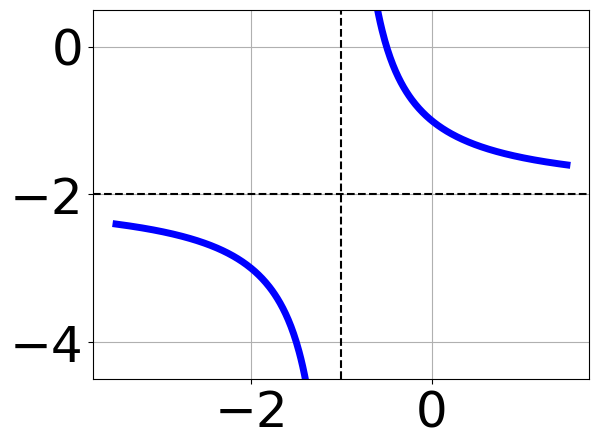
\includegraphics[width=0.3\textwidth]{../Figures/rationalEquationToGraphCopyDA.png}
\end{center}\begin{enumerate}[label=\Alph*.]
\begin{multicols}{2}
\item 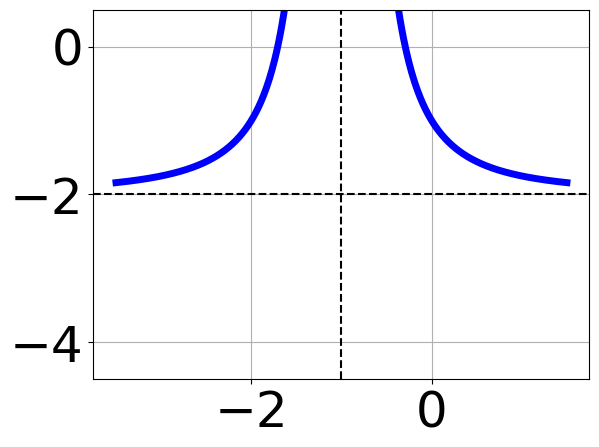
\includegraphics[width = 0.3\textwidth]{../Figures/rationalEquationToGraphCopyAA.png}
\item 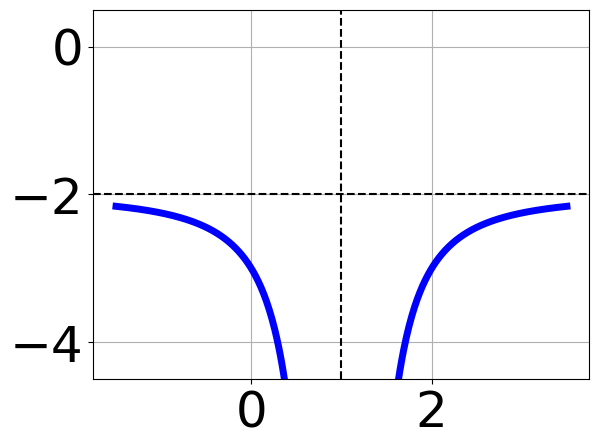
\includegraphics[width = 0.3\textwidth]{../Figures/rationalEquationToGraphCopyBA.png}
\item 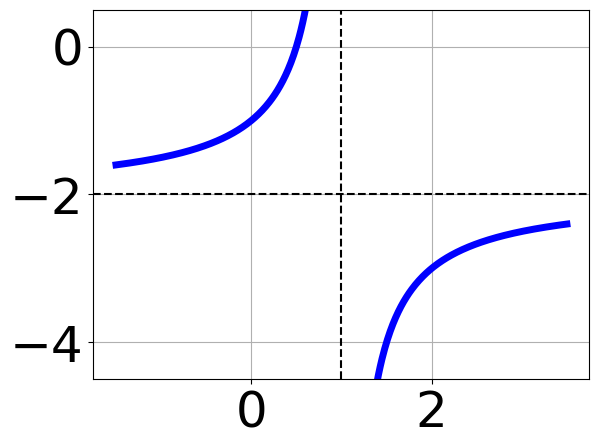
\includegraphics[width = 0.3\textwidth]{../Figures/rationalEquationToGraphCopyCA.png}
\item 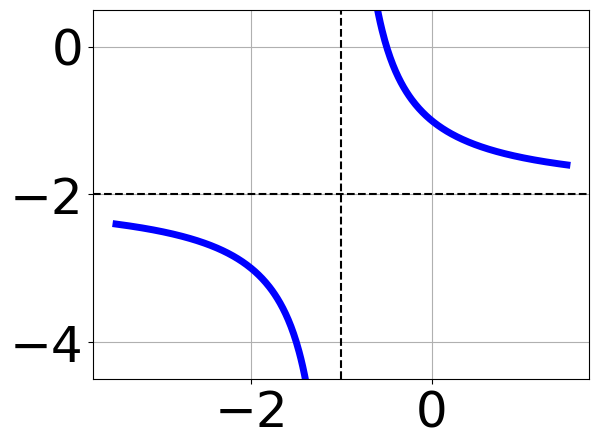
\includegraphics[width = 0.3\textwidth]{../Figures/rationalEquationToGraphCopyDA.png}
\end{multicols}\item None of the above.\end{enumerate}
\textbf{General Comment:} Remember that the general form of a basic rational equation is $ f(x) = \frac{a}{(x-h)^n} + k$, where $a$ is the leading coefficient (and in this case, we assume is either $1$ or $-1$), $n$ is the degree (in this case, either $1$ or $2$), and $(h, k)$ is the intersection of the asymptotes.
}
\litem{
Choose the equation of the function graphed below.

\begin{center}
    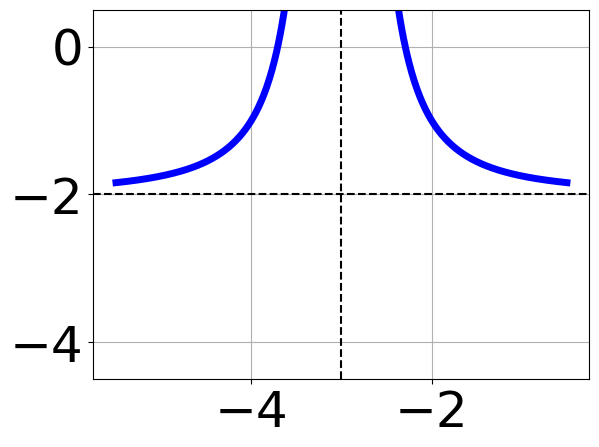
\includegraphics[width=0.5\textwidth]{../Figures/rationalGraphToEquationCopyA.png}
\end{center}


The solution is \( f(x) = \frac{1}{(x + 3)^2} - 2 \), which is option A.\begin{enumerate}[label=\Alph*.]
\item \( f(x) = \frac{1}{(x + 3)^2} - 2 \)

This is the correct option.
\item \( f(x) = \frac{-1}{(x - 3)^2} - 2 \)

Corresponds to using the general form $f(x) = \frac{a}{(x+h)^2}+k$ and the opposite leading coefficient.
\item \( f(x) = \frac{1}{x + 3} - 2 \)

Corresponds to thinking the graph was a shifted version of $\frac{1}{x}$.
\item \( f(x) = \frac{-1}{x - 3} - 2 \)

Corresponds to thinking the graph was a shifted version of $\frac{1}{x}$, using the general form $f(x) = \frac{a}{(x+h)^2}+k$, and the opposite leading coefficient.
\item \( \text{None of the above} \)

This corresponds to believing the vertex of the graph was not correct.
\end{enumerate}

\textbf{General Comment:} Remember that the general form of a basic rational equation is $ f(x) = \frac{a}{(x-h)^n} + k$, where $a$ is the leading coefficient (and in this case, we assume is either $1$ or $-1$), $n$ is the degree (in this case, either $1$ or $2$), and $(h, k)$ is the intersection of the asymptotes.
}
\litem{
Choose the graph of the equation below.
\[ f(x) = \frac{-1}{(x + 2)^2} - 2 \]The solution is the graph below, which is option D.
\begin{center}
    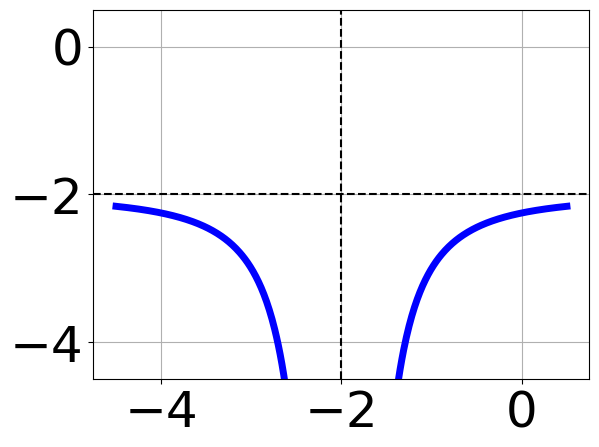
\includegraphics[width=0.3\textwidth]{../Figures/rationalEquationToGraphDA.png}
\end{center}\begin{enumerate}[label=\Alph*.]
\begin{multicols}{2}
\item 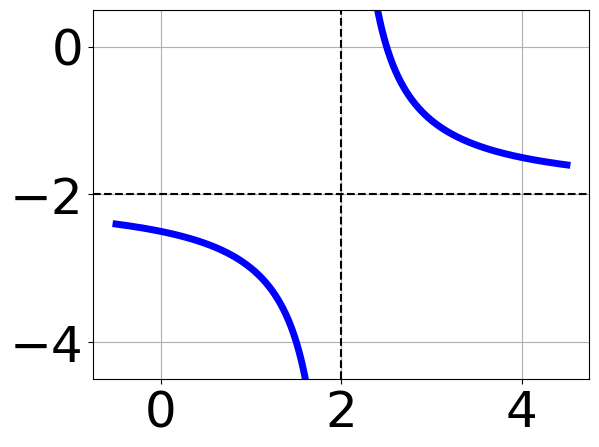
\includegraphics[width = 0.3\textwidth]{../Figures/rationalEquationToGraphAA.png}
\item 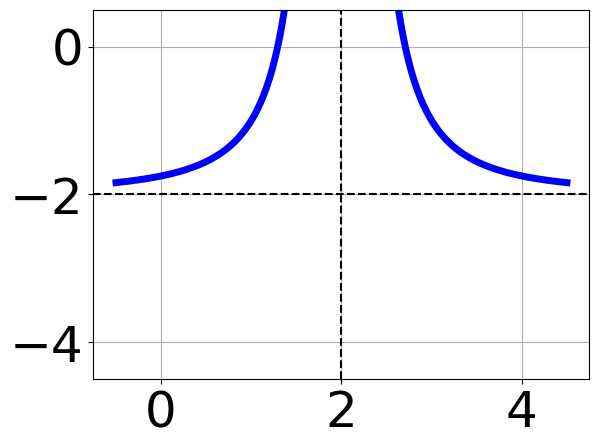
\includegraphics[width = 0.3\textwidth]{../Figures/rationalEquationToGraphBA.png}
\item 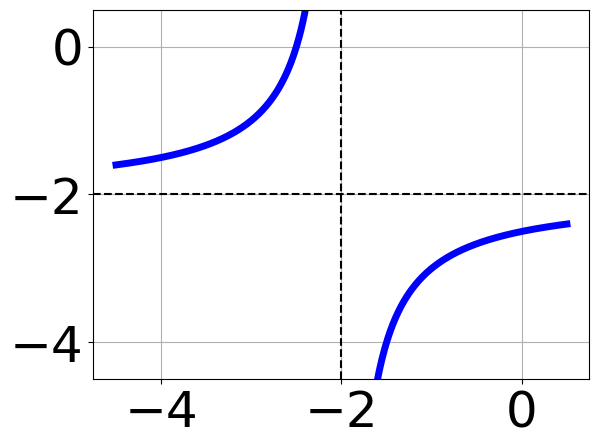
\includegraphics[width = 0.3\textwidth]{../Figures/rationalEquationToGraphCA.png}
\item 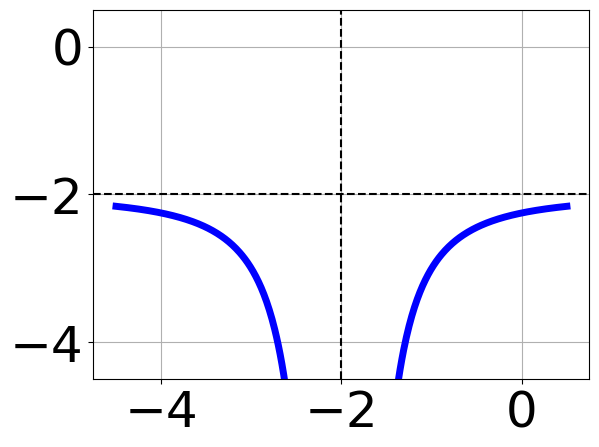
\includegraphics[width = 0.3\textwidth]{../Figures/rationalEquationToGraphDA.png}
\end{multicols}\item None of the above.\end{enumerate}
\textbf{General Comment:} Remember that the general form of a basic rational equation is $ f(x) = \frac{a}{(x-h)^n} + k$, where $a$ is the leading coefficient (and in this case, we assume is either $1$ or $-1$), $n$ is the degree (in this case, either $1$ or $2$), and $(h, k)$ is the intersection of the asymptotes.
}
\litem{
Solve the rational equation below. Then, choose the interval(s) that the solution(s) belongs to.
\[ \frac{3}{-4x + 7} + -7 = \frac{-3}{-20x + 35} \]The solution is \( x = 1.621 \), which is option A.\begin{enumerate}[label=\Alph*.]
\item \( x \in [1.62,2.62] \)

* $x = 1.621$, which is the correct option.
\item \( x_1 \in [-1.94, -1.82] \text{ and } x_2 \in [1.62,3.62] \)

$x = -1.879 \text{ and } x = 1.621$, which corresponds to getting the correct solution and believing there should be a second solution to the equation.
\item \( x_1 \in [1.49, 1.62] \text{ and } x_2 \in [1.62,3.62] \)

$x = 1.536 \text{ and } x = 1.621$, which corresponds to getting the correct solution and believing there should be a second solution to the equation.
\item \( x \in [-1.94,-1.82] \)

$x = -1.879$, which corresponds to not distributing the factor $-4x + 7$ correctly when trying to eliminate the fraction.
\item \( \text{All solutions lead to invalid or complex values in the equation.} \)

This corresponds to thinking $x = 1.621$ leads to dividing by zero in the original equation, which it does not.
\end{enumerate}

\textbf{General Comment:} Distractors are different based on the number of solutions. Remember that after solving, we need to make sure our solution does not make the original equation divide by zero!
}
\litem{
Solve the rational equation below. Then, choose the interval(s) that the solution(s) belongs to.
\[ \frac{-6x}{-7x -3} + \frac{-5x^{2}}{42x^{2} -24 x -18} = \frac{-4}{-6x + 6} \]The solution is \( \text{There are two solutions: } x = -0.173 \text{ and } x = 2.238 \), which is option A.\begin{enumerate}[label=\Alph*.]
\item \( x_1 \in [-0.94, 0.1] \text{ and } x_2 \in [0.2,3.1] \)

* $x = -0.173 \text{ and } x = 2.238$, which is the correct option.
\item \( x \in [0.59,1.17] \)


\item \( x_1 \in [-0.94, 0.1] \text{ and } x_2 \in [-2.5,0.8] \)


\item \( x \in [1.58,2.73] \)


\item \( \text{All solutions lead to invalid or complex values in the equation.} \)


\end{enumerate}

\textbf{General Comment:} Distractors are different based on the number of solutions. Remember that after solving, we need to make sure our solution does not make the original equation divide by zero!
}
\litem{
Determine the domain of the function below.
\[ f(x) = \frac{6}{15x^{2} +48 x + 36} \]The solution is \( \text{All Real numbers except } x = -2.000 \text{ and } x = -1.200. \), which is option A.\begin{enumerate}[label=\Alph*.]
\item \( \text{All Real numbers except } x = a \text{ and } x = b, \text{ where } a \in [-2.81, -1.6] \text{ and } b \in [-1.38, -0.99] \)

All Real numbers except $x = -2.000$ and $x = -1.200$, which is the correct option.
\item \( \text{All Real numbers except } x = a, \text{ where } a \in [-2.81, -1.6] \)

All Real numbers except $x = -2.000$, which corresponds to removing only 1 value from the denominator.
\item \( \text{All Real numbers except } x = a \text{ and } x = b, \text{ where } a \in [-30.07, -29.63] \text{ and } b \in [-18.33, -17.26] \)

All Real numbers except $x = -30.000$ and $x = -18.000$, which corresponds to not factoring the denominator correctly.
\item \( \text{All Real numbers except } x = a, \text{ where } a \in [-30.07, -29.63] \)

All Real numbers except $x = -30.000$, which corresponds to removing a distractor value from the denominator.
\item \( \text{All Real numbers.} \)

This corresponds to thinking the denominator has complex roots or that rational functions have a domain of all Real numbers.
\end{enumerate}

\textbf{General Comment:} Recall that dividing by zero is not a real number. Therefore the domain is all real numbers \textbf{except} those that make the denominator 0.
}
\litem{
Solve the rational equation below. Then, choose the interval(s) that the solution(s) belongs to.
\[ \frac{7}{-7x + 2} + -4 = \frac{2}{14x -4} \]The solution is \( x = -0.000 \), which is option B.\begin{enumerate}[label=\Alph*.]
\item \( x \in [-1.07,-0.45] \)

$x = -0.571$, which corresponds to not distributing the factor $-7x + 2$ correctly when trying to eliminate the fraction.
\item \( x \in [-1.0,1.0] \)

* $x = -0.000$, which is the correct option.
\item \( x_1 \in [-1.07, -0.45] \text{ and } x_2 \in [-0.24,0.04] \)

$x = -0.571 \text{ and } x = -0.000$, which corresponds to getting the correct solution and believing there should be a second solution to the equation.
\item \( x_1 \in [-0.52, 0.2] \text{ and } x_2 \in [0.08,0.19] \)

$x = -0.000 \text{ and } x = 0.107$, which corresponds to getting the correct solution and believing there should be a second solution to the equation.
\item \( \text{All solutions lead to invalid or complex values in the equation.} \)

This corresponds to thinking $x = -0.000$ leads to dividing by zero in the original equation, which it does not.
\end{enumerate}

\textbf{General Comment:} Distractors are different based on the number of solutions. Remember that after solving, we need to make sure our solution does not make the original equation divide by zero!
}
\litem{
Solve the rational equation below. Then, choose the interval(s) that the solution(s) belongs to.
\[ \frac{5x}{3x -5} + \frac{-6x^{2}}{-9x^{2} -3 x + 30} = \frac{4}{-3x -6} \]The solution is \( \text{There are two solutions: } x = 0.397 \text{ and } x = -2.397 \), which is option E.\begin{enumerate}[label=\Alph*.]
\item \( \text{All solutions lead to invalid or complex values in the equation.} \)


\item \( x \in [-2.3,-1.44] \)


\item \( x_1 \in [-0.36, 1.22] \text{ and } x_2 \in [-0.33,2.67] \)


\item \( x \in [-3.05,-2.04] \)


\item \( x_1 \in [-0.36, 1.22] \text{ and } x_2 \in [-4.4,1.6] \)

* $x = 0.397 \text{ and } x = -2.397$, which is the correct option.
\end{enumerate}

\textbf{General Comment:} Distractors are different based on the number of solutions. Remember that after solving, we need to make sure our solution does not make the original equation divide by zero!
}
\litem{
Choose the equation of the function graphed below.

\begin{center}
    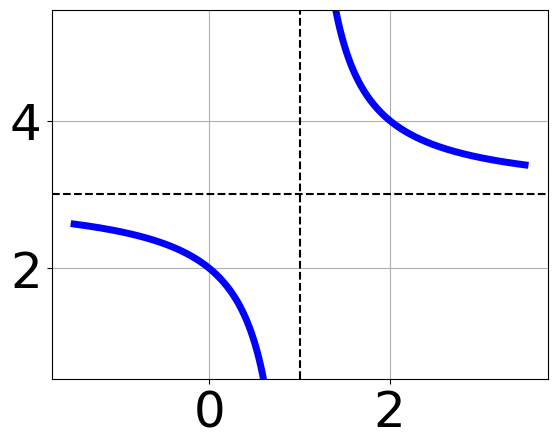
\includegraphics[width=0.5\textwidth]{../Figures/rationalGraphToEquationA.png}
\end{center}


The solution is \( f(x) = \frac{1}{x - 1} + 3 \), which is option D.\begin{enumerate}[label=\Alph*.]
\item \( f(x) = \frac{1}{(x - 1)^2} + 3 \)

Corresponds to thinking the graph was a shifted version of $\frac{1}{x^2}$.
\item \( f(x) = \frac{-1}{(x + 1)^2} + 3 \)

Corresponds to thinking the graph was a shifted version of $\frac{1}{x^2}$, using the general form $f(x) = \frac{a}{x+h}+k$, and the opposite leading coefficient.
\item \( f(x) = \frac{-1}{x + 1} + 3 \)

Corresponds to using the general form $f(x) = \frac{a}{x+h}+k$ and the opposite leading coefficient.
\item \( f(x) = \frac{1}{x - 1} + 3 \)

This is the correct option.
\item \( \text{None of the above} \)

This corresponds to believing the vertex of the graph was not correct.
\end{enumerate}

\textbf{General Comment:} Remember that the general form of a basic rational equation is $ f(x) = \frac{a}{(x-h)^n} + k$, where $a$ is the leading coefficient (and in this case, we assume is either $1$ or $-1$), $n$ is the degree (in this case, either $1$ or $2$), and $(h, k)$ is the intersection of the asymptotes.
}
\end{enumerate}

\end{document}